\section{Dane}
\label{sec:dane}

% [MWI] Dwa główne cele opisane w~sub sekcjach: 
% 1. raport z~dostępnych baz danych 
% 2. utworzona baza

\subsection{Dostępne bazy}

Tu piszemy ogólny komentarz o dostępnych bazach danych.... Jeśli jest jedna to ten rozdział można zmieścić jako ostatni podrozdział wstępu po przeglądzie literatury.

\subsubsection{Baza 1}

Tu już konkretnie o bazie 1 użytej do testu z referencją do niej. Warto wskazać wady i zalety tej bazy.

\subsubsection{Baza 2}

Tu już konkretnie o bazie 1 użytej do testu z referencją do niej. Warto wskazać wady i zalety tej bazy.


\subsection{Utworzona baza nagrań}

Jeśli jakaś powstała można ją tu opisać

\subsubsection*{Proces tworzenia bazy}

Jakim sprzętem nagrywano, jakie nastawy sprzętu zastosowano, dlaczego takie. Procedura nagrań itp. 

\subsubsection*{Parametry techniczne bazy}

Jako efekt podstawowej obróbki uzyskano bazę nagrań o~następujących parametrach:
\begin{itemize}
  \setlength\itemsep{-0.25em}
  \item Nazwa bazy: Speech Dataset,
  \item Liczba nagrań: 529,
  \item Liczba nagranych osób: 15,
  \item Minimalna długość nagrania: 8 sekund,
  \item Maksymalna długość nagrania: 23 sekundy,
  \item Częstotliwość próbkowania nagrań: 44100 Hz,
  \item Głębia bitowa: 24 bity na próbkę,
  \item Liczba kanałów: 1,
  \item Format plików: WAV.
\end{itemize}

Histogram długości plików w~bazie nagrań przedstawiono na rysunku \ref{rysunek:histogram_gsd}.

\begin{figure}[H]
    \centering
    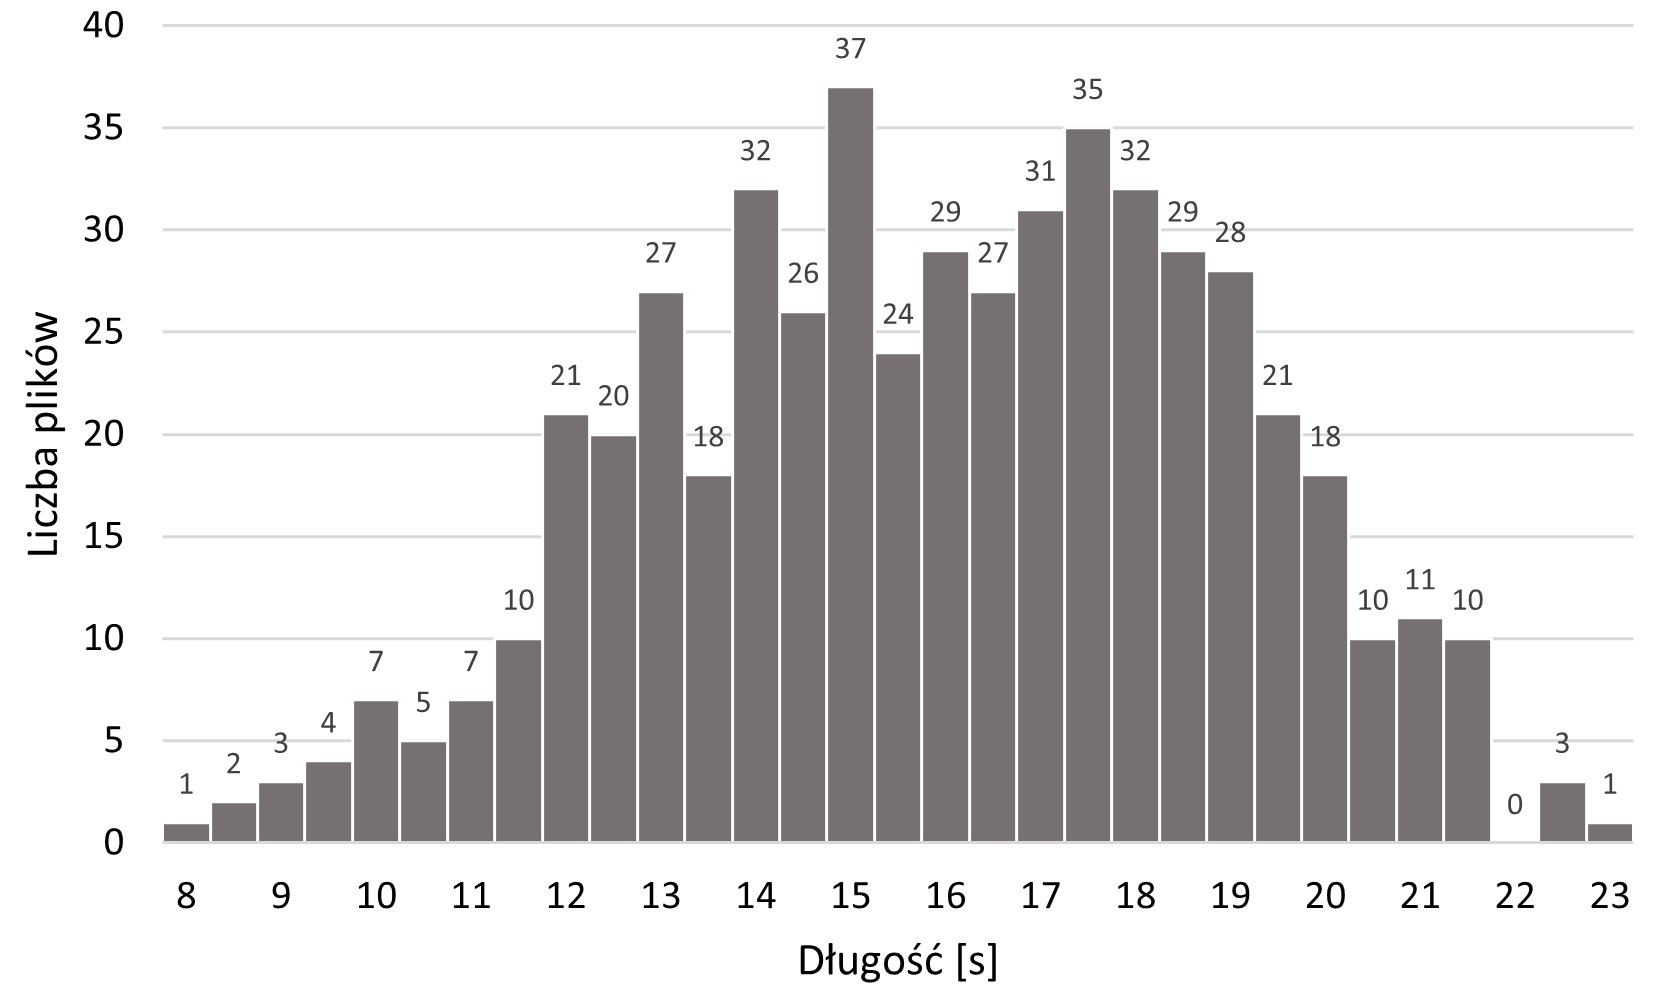
\includegraphics{img/histogram_gsd.jpg}
    \caption{Histogram długości nagrań w~bazie Speech Dataset.}
    \label{rysunek:histogram_gsd}
\end{figure}

\subsubsection*{Etykietowanie bazy}

Jak wyglądało etykietowanie bazy danych.